\documentclass{proc}
\usepackage{graphicx}
\graphicspath{ {./} }
\begin{document}

\title{Real-time Visualization of a Distributed Peer-to-Peer Botnet}

\author{Alejandro Soler Gayoso, Rushdi Abualhaija}

\maketitle

\section{Introduction}
Botnets stand out as one of the largest security threats to the average user. Composed sometimes by tens of thousands of nodes, they can collectively perform massive coordinated attacks, such as Distributed Denial of Service. Traditionally, bots in the network receive their commands from Command and Control (C&C) servers, which produced malicious commands camouflaged in regular network traffic. 


It is no easy task to bring down one of these nefarious networks, especially as the size of the botnet increases. Taking down one individual node will not serve any purpose, as there could be thousands of others still at work. However, if the C&C server were to be compromised, it could lead to the downfall of the entire botnet. However, the rise of a new type of botnet built on a distributed peer-to-peer (p2p) architecture are resilient to this approach since commands are not distributed from a single C&C server, but rather from each node to its neighbors and so on. 


Effectively controlling these type of networks can be a rather overwhelming task. In an stealthy p2p botnet, traffic should always take different routes, and commands should come from different origins, making the management quite a tedious and leading to inefficient routes, and partial command propagation. For that reason, we are proposing a visualization of a p2p botnet on real-time, that would optimize the its management by providing an overall view of the topology, as well as route statistics, for better propagation. 

\section{One-sentence description}
Optimizing control and analysis of a distributed peer-to-peer botnet can be achieved by visualizing the state of the network through different coordinated views depicting real-time data.
\section{Project Type}
Real-Time Simulation
\section{Audience} 
Security researchers are always looking for ways to better understand, detect, and neutralize hostile botnets. Botnets are extremely prevalent today and have already caused untold damage with their DDoS attacks and ability to silently infect and perform actions from within countless hosts. For example in 2008 the Kraken botnet was found to be present within 10\% of all fortune 500 companies and was capable of sending over 600,000 emails a day. Another aspect that makes botnets risky is the range of threats from malicious actors to bored kids such as in the case of the 2016 Mirai botnet which infected over 600,000 machines and used to DDoS attacks to make the internet inacessible to most users on the east coast. This attack was put together by a group of kids looking to have an advantage in a videogame\cite{WhiteOps}. Security researchers looking to understand data dissemination within a hostile botnet will find this tool valuable as they can run simulations with visualizations that could make patterns of a botnet spreading that could reveal patterns of how botnets spread and help develop methods to stem the spreading of these infectious botnets. Additionally, security researchers can use this tool to collect data about how botnets run and  the way that commands and information are passed between them allowing for easier development of detection tools. If this problem remains unsolved botnets will continue to cause damage by infecting users computers and causing malicious attacks.

\section{Approach}
\subsection{Details}

It is quite a difficult task to manage a network as its size increases, and such complexity multiples with a peer-to-peer architecture. Nowadays, an example of a The goal is to ease the management of a distributed network. Visualizing the real-time flow of a peer-to-peer network using a network graph-style approach, synchronized with other views. This would provide the user with a big picture of the network, and the state of all the nodes, as well as different statistics of the edges. Hence, allowing such user to take better and faster decisions, such as changing routes, or the topology of the network itself.

Other approaches we have also considered include an chord of interconnected nodes focusing on the most relevant links to avoid overcrowding it with lines, see figure 1. However, this might not be the most scalable approach, as it might be useful to spot big trends, but not to interact with individual nodes and links. 

\begin{figure}
  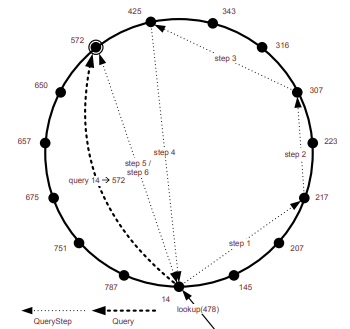
\includegraphics[width=\linewidth]{net_map.png}
  \caption{Chord of a P2P botnet with relevant links.}
  \label{fig1 :boat1}
\end{figure}

\subsection{Evidence for Success}

There are similar models in place that allow network engineers to visualize the state of the network they are managing. We believe that applying a similar approach to p2p architectures will not only be a great tool for network managers, but also for security researchers studying distributes p2p botnets. 

\section{Best-case Impact Statement}

In the best case scenario, our project would accurately represent the state of a p2p botnet on real-time, along with network link statistics. Additionally, it would allow the user quickly spot any anomalies or settings in the network, and change them through interactive features. Ultimately, we see this project as a potential foundation for future work in distributed architectures visualization. If successful, further development could be done to improve efficiency and reliability of the visualization. 
\section{Major Milestones}
\begin{itemize}
\item Accurately visualize real-time data produce by a peer-to-peer botnet.
\item Interact with specific nodes of the network and preform actions such as submitting commands.
\item Tracking the flow and direction of packet in the network.
\item Display the the geo-location of a node on a map.
\item Gather and visualize network statistics such as latency and jitter on the edges, as well as the state of the nodes.
\end{itemize}

\section{Obstacles}

\subsection{Major obstacles} % (if these fail, the project is over)
\begin{itemize}
\item Simulating a botnet requires a peer-to-peer network application that can coordinate its actions and that also has a method of controlling the bots in the network. This is a technically difficult application to create.
\item Creating an interactive visualization tool that successfully presents the features of the botnet in a way that is constructive to finding patterns and generating data will be difficult as we will need to put considerable thought into the features that such a tool will require to be succesful.

\end{itemize}

\subsection{Minor obstacles}

\begin{itemize}
\item Creating a sizable number of nodes in the botnet will require a good amount of computing resources that we don't have readily accessible. To circumvent this we can write a script to generate our own data. 
\end{itemize}
\section{Resources Needed}
\begin{itemize}
\item Code to generate our own data to successfully simulate a peer-to-peer botnet
\item Back end botnet application
\end{itemize}

\section{5 Related Publications}

\begin{itemize}

\item{Junemann et. al created OvlVis, a visualization tool for P2P network development. OvlVis is capable of creating a simulation of a P2P network, as well as the communication between the nodes.It Moreover, OvlVis is capable of visualizing processes on multiple layers. \cite{ovlvis}}

\item{Allcock et. al developed GridMapper, a tool for registering data to physical locations and then automatically laying it out on a map. It also provides tools for animating these data points and resources and how they change based on their activities. This is similar to how we want to visualize the distributed peer-to-peer network and the flow of network traffic across it.\cite{gridmapper}}

\item{Conti et. al developed a framework for designing security visualizations. They additionally created two systems with this tool and surveyed security experts on the efficacy of the tools they created. Their surveys showed that this type of interactive visualization presented a significant advantage to security analysts over traditional text based analysis tools.\cite{packet_vis}}

\item{Gray et. al proposes to use contextual navigation to provide situational awareness for the user. Instead of plotting all the nodes and link on the same relative location, a context-based navigation would present a different location for every location, representing the "best" route from the location to all the others.\cite{context_net}}

\item{Krasser et. al wrote about the limitations of just having human analysis of network traffic to detect anomalies in that the volume of traffic is too great for a human to analyze. Additionally they covered how automatic techniques generate an unacceptable number of false positives and false negatives. Krasser et. al developed a tool to allow human and automatic processes to achieve better detection margins, and they showed that this approach in fact works.\cite{real_time}}


\end{itemize}


\section{Define Success}

For this to be considered successful we need to have produced a tool that is capable of generating realistic botnet traffic, and an overlying visualization tool that is capable of inspecting various aspects of that network. This includes the amount and type of data being sent between nodes in the network.



\nocite{*}

\bibliographystyle{abbrv}
\bibliography{prospectus}


\end{document}





